\documentclass[../../main.tex]{subfiles}
    
    \lstset{basicstyle=\small,
      showstringspaces=false,
      commentstyle=\color{black},
      keywordstyle=\color{blue}
    }
    
    \graphicspath{{images/Konzepte/}{../../images/Konzepte/}}


    \begin{document}
    \subsection{Ablauf} \label{ablauf}
    Dieses Kaptiel gibt eine Übersicht über den Gesammten Ablauf, der nötig ist um die Aufgabenstellung zu erfüllen. Der Ablauf ist in \ref{fig:Ablaufdiagramm} Grafisch dargestellt. Der Ablauf kann in fünf Zustände unterteilt werden.\\

    \begin{figure}
        \centering
        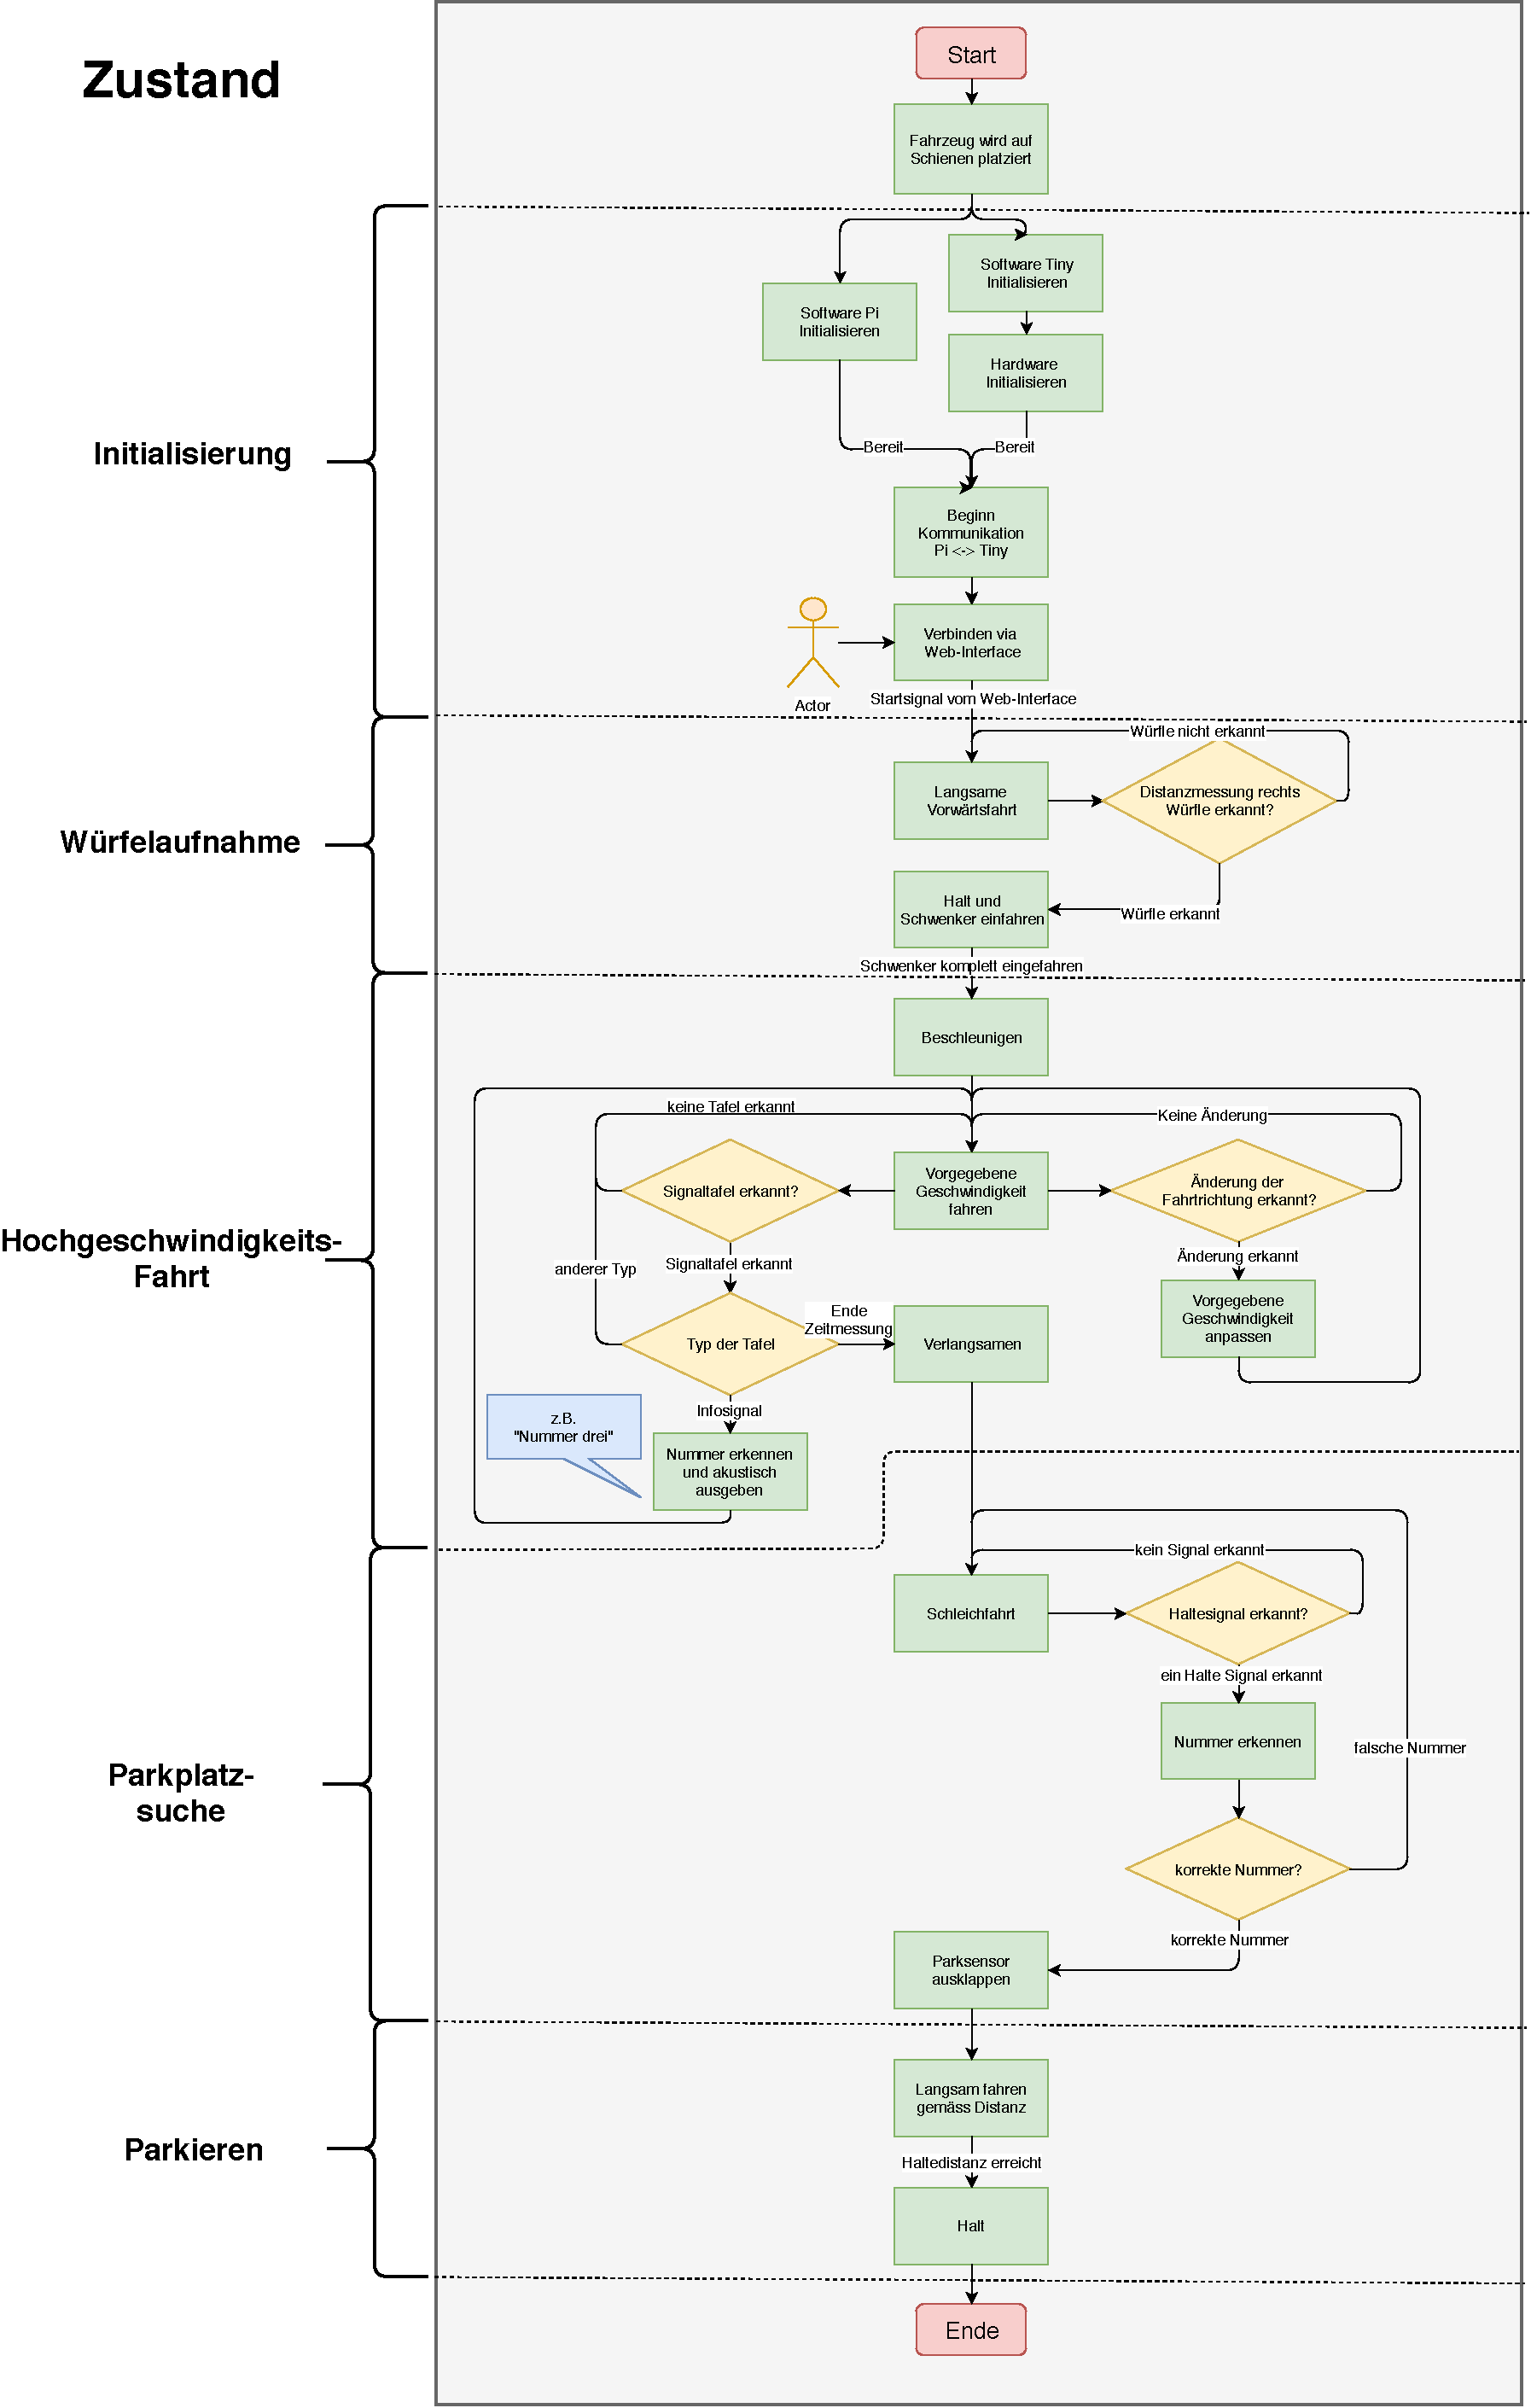
\includegraphics[width=1.0\textwidth]
        {../../drawings/Ablaufdiagramm/Ablaufdiagramm.pdf}
        \caption {Ablaufdiagramm}
        \label{fig:Ablaufdiagramm}
    \end{figure}

    \begin{itemize}
        \item Initialisierung
        \item Würfelaufnahem
        \item Hochgeschwindigkeitsfahrt
        \item Parkplatzsuche
        \item Parkieren
    \end{itemize}

    Im folgenden werden die Zustände kurz beschrieben.\\

    \textbf{Initialisierung}\\
    Alle Systeme werden Gestartet sobald sie mit Strom versorgt werden. Alle Schnittstellen werden Initialisiert und die Kommunikation beginnt. Beim Ende der Initialisierung soll über das Web Interface angezeigt werden, dass das System bereit ist und die Fahrt gestartet werden kann.\\

    \textbf{Würfleaufnahme}\\
    Nach dem Startsignal über das Web Interface fährt der Zug in langsamer Fahrt vorwärts bis der Würfle von den Sensoren erfasst wird. Sobald der Würfel erkannt wurde hält der Zug an und der Schwenker mit dem Würfel wird eingefahren.\\

    \textbf{Hochgeschwindigkeitsfahrt}\\
    Nachdem der Würfel Aufgeladen ist kann der Zug beschleunigen. Der Zug soll immer die Höchstmögliche Geschwindigkeit fahren. Die Geschwindigkeit wird für die Kurven gemäss der Bilderkennung angepasst. Auch sucht das System dauernd das Infosignal und erkennt die Nummer darauf, sobald die Nummer erkannt wurde gibt das System diese Information über den Lautsprecher aus. 
    Sobald das Signal der Ende der Zeitmessung erkannt wird verlangsamt der Zug und beginnt die Parkplatzsuche\\

    \textbf{Parkplatzsuche}\\
    Um das korrekte Haltesignal zu finden kann der Zug eine so tiefe Geschwindigkeit fahren wie nötig. Die Bilderkennung sucht das korrekte Signal und entscheidet wo der Zug parkiert werden soll.\\

    \textbf{Parkieren}\\
    Nachdem das korrekte Signal erkannt ist, wird der Parksensor ausgeklappt. Dieser misst die Distanz zum Haltesignal bis ein bestimmter Schwellwert erreicht ist. Beim Erreichen der Haltedistanz Stoppt der Zug und beendet damit die Fahrt.

    \end{document}